\documentclass[reprint,norsk,notitlepage]{revtex4-2}
\usepackage{amsmath}
\usepackage[mathletters]{ucs}
\usepackage[utf8x]{inputenc}
\usepackage[norsk]{babel}
\usepackage{esint}
\usepackage{physics,amssymb}
\usepackage{graphicx}
\usepackage{xcolor}
\usepackage[colorlinks]{hyperref}
\usepackage{cleveref}
\usepackage{listings}
\usepackage{subfig}
\usepackage{booktabs}
\usepackage{caption}
\usepackage{listings}



\begin{document}

\title{Lab Rapport - Masse}
\author{Oskar Idland}
\affiliation{University of Oslo}
\date{}


\begin{abstract}
\textit{I dette eksperimentet prøvde vi forskjellige måter å måle masse og små masseendringer. Vi gjorde dette via en bladfjær med måleur, en harmonisk oscillator og bladfjær med en laser. Resultatene variert og bladfjær med måleur var en klar vinner. }
\end{abstract}
\maketitle

\section{Introduksjon} \label{sec: introduction}
Masse er en en ekstremt viktig størrelse i fysikken ettersom det er en grunnstørrelse og grunnenhet i SI systemet. Det betyr at vi bruker masse til å bygge opp andre fysiske størrelser. Dette gjør det vesentlig å ha en felles forståelse for hva for eksempel et kilogram er. Vi må også klare å måle dette på en måte som er nøyaktig reproduser bar. I denne rapporten skal vi utforske forskjellige måter å måle masse på, og se på hvor nøyaktig disse målingene er og hvor små endringer i vekt $Δm$ (følsomhet), vi kan detektere. Vi bruker elastisk deformasjon i en bladfjær med et måleur, en harmonisk oscillator og bladfjær med refleksjon av laser stråle. Objektet som skal veies er et aluminiums lodd.

\section{Teori} \label{sec: theory}
\subsection{Numerisk Lineær Regresjon} \label{ssec: linear regression}
Ved bruk av Python kan vi gjøre en numerisk lineær regresjon basert på dataen vi samler iløpet av eksperimentet. Dette gjør vi ved å bruke biblioteket \texttt{scipy.stats.linregress} som tar inn to lister med x og y verdier. Denne funksjonen gir oss en modell vi kan hente ut stigningstallet $a$, konstanten $b$, standardavviket til stigningstallet $Δa$ og standardavviket til konstanten $Δb$. Dette vil brukes til å finne en lineær funksjon som kan brukes til å beregne massen til et objekt og vil være på formen 
\begin{equation}\label{eq: linear regression}
    m(l) = a ⋅ l + b.
\end{equation}

\subsection{Usikkerhet} \label{ssec: uncertainty}
Når vi regner på usikkerheter er de mest relevante i form av menneskelige feil (avlesning av instrumenter eller forskjell i oppsett), og usikkerheten i instrumentene brukt. Ofte er det en kombinasjon av usikkerheter fra instrumentene og menneskelige feil som gir den totale usikkerheten. Den totale usikkerheten $ΔZ$ kan vi beregne ut fra de uavhengige usikkerhetene $ΔA$ og $ΔB$. 
\begin{equation}\label{eq: uncertainty sum}
    ΔZ = \sqrt{ΔA^2 + ΔB^2}.
\end{equation}
 

For å redusere usikkerheten i målingene gjør vi dette flere ganger, tar gjennomsnittet av målingene og regner ut standardavviket til gjennomsnittet, også kjent som standard error in the mean (SE). 


\subsection{Standardavvik til midlere verdi}
Ved en måling $x$ vil vi få den usikkerhet $Δx$ som er gitt av standardavviket til målingen. Gjør vi flere målinger må vi regne på hvert enkelt standardavvik for å finne standardavviket til gjennomsnittsverdien $SE(\left<x\right>)$ gitt ved 
\begin{equation}\label{eq: SE}
    SE(\left<x\right>) = \frac{Δx}{\sqrt{n}} = Δ\left<x\right>. 
\end{equation}


\subsection{Måleur}
Måleuret har en liten nål i bunn som kan bevege seg opp og ned. Selve uret lar oss lese av dette i $0.01$ mm. Dette har en usikkerhet som vi skal ta med i beregningene. Den totale usikkerheten $Δl$ i lengden avlest er gitt av usikkerheten i instrumentet $Δl_i$, avlesning $Δl_a$  og standard error in the mean $SE(\left<l\right>)$, der $\left<l\right>$ er gjennomsnittslengden målt. Måleuret brukt (nr. B1232)
har en usikkerhet vi leser av i databladet i \cref{fig: datablad maaleur} 

Dette gir en total usikkerhet $Δl_t$ på 
\begin{equation}\label{eq: total length uncertainty}
    Δl = \sqrt{\underbrace{Δl_i^2 + Δl_a^2}_{\text{Riktighet}} + \underbrace{SE(\left<l\right>)^2}_{\text{Presisjon}}}.
\end{equation}

Når vi skal finne den minste massen vi kan måle $Δm$ tar vi også hensyn til riktigheten og presisjonen. Her er $a$ stigningstallet til linjen produsert av den numeriske lineær regresjonen av dataen og $Δa$ dets tilhørende usikkerhet. Samme gjelder for $b$ og $Δb$ som er konstanten i lineær regresjonen som definert i seksjon \ref{ssec: linear regression}. $Δl$ er den totale usikkerheten i lengden som vi fant via \cref{eq: total length uncertainty}.
\begin{equation}\label{eq: mass uncertainty}
    Δm = \sqrt{\underbrace{\left(\left<l\right> ⋅ Δa\right)^2 + \left(Δb\right)^2}_{\text{Riktighet}} + \underbrace{\left(a ⋅ Δl_t\right)^2}_{\text{presisjon}}}  
\end{equation}

Vi har også en alternativ formel som kan brukes for å finne den minste massen vi kan måle i en harmonisk oscillator. Denne formelen er gitt ved
\begin{equation}\label{eq: mass uncertainty alternative}
    Δm = \frac{2mΔτ}{τ}  
\end{equation}
hvor $τ$ er svingeperioden og $Δτ$ dets usikkerhet. 

\subsection{Dynamisk Område}
Det dynamiske område til et instrument er det området hvor instrumentet vil gi en nøyaktig måling. Dette er gitt av en kombinasjon av usikkerhetene i instrumentet, hvilket område det er kalibrert for og våre krav til dets presisjon. Ta for eksempel en vekt som er kalibrert mellom 0 og 100 g, men som har en usikkerhet på 5 g. Hvis vi ønsker oss en presisjon på 5 g vil vekten duge akkurat i intervallet fra 5 til 95 g eller to størrelsesordener. Hvis vi ønsker oss en presisjon på 10\% ville vekten hatt dynamisk område på 55 til 95 g. Dynamisk område er altså avhengig av både instrumentet og kravene til presisjonen.
  
\section{Metode} \label{sec: method} 
\subsection{Bladfjær og Måleur}
\subsubsection{Oppsett} \label{ssec: setup maaleur}

\begin{figure}[h!]
  \centering
  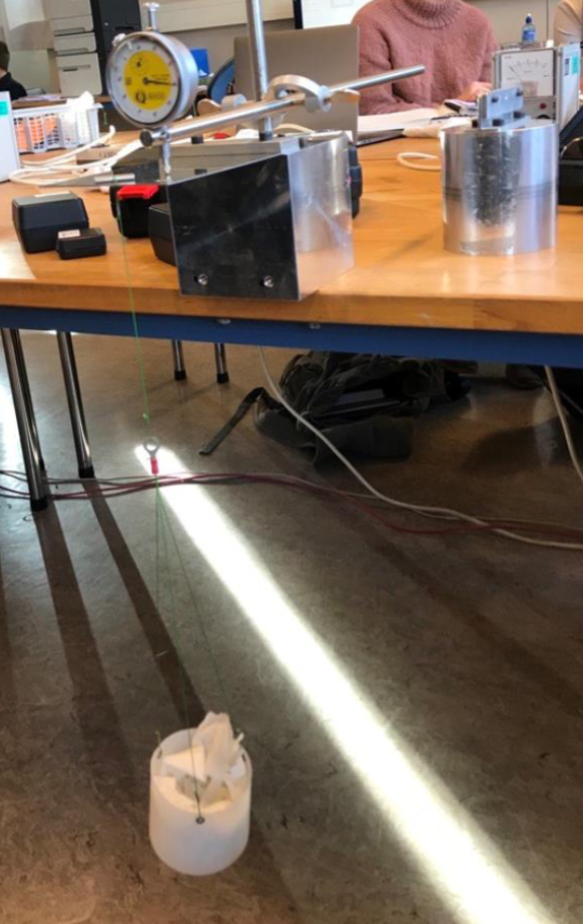
\includegraphics[width = 0.25\textwidth]{fig/maaleur_oppsett.png}
  \caption{Oppsett av bladfjær og måleur}
  \label{fig: oppsett maaleur}
\end{figure}

Bladfjæren er festet med to skruer, horisontalt til en blokk med aluminium, slik at den får svinge vertikalt. I et hull i ytterst på bladfjæren festes en tråd med en kurv i enden (se \cref{fig: oppsett maaleur}). På aluminiums blokken er det festet en stang som holder måleuret. Ettersom bladfjæren vil bli trukket nedover mot vekten må måleuret sin nål være betydelig sammentrukket for å forsikre oss om at den har nok lengde til å ha kontakt med bladfjæren. Vi fester måleuret så langt ute på fjæren som mulig slik at vi får størst mulig spenn i målt lengde. For å forsikre oss om at vi har nok lengde å spille på setter vi aluminiums loddet, som vi vet er circa det tyngste vi skal veie, og ser at nålen til uret har nok lengde til å nå bladfjæren.
\paragraph{\bf Intensjon:}
Når vi legger på vekt vil bladfjæren bli trukket nedover sammen med nålen på måleuret. Dette vil la oss lage en lineærtilpassing av målt lengde mot vekt. 


\subsubsection{Måling} \label{ssec: measurement maaleur}
For å kunne bruke deformasjonene i bladfjæreren samt måleuret til å måle massen til et objekt må vi først kalibrere vekten vår. Dette gjør vi ved å legge en rekke kombinasjoner av 4 typer kalibrerings lodd på 500 g, 100 g, 10 g og 1 g. Vi legger disse loddene i kurven i enden av bladfjæren og noterer både masse og utslag $l$ på måleuret som en ser i \cref{tab: maaleur and laser results}. Vi banker i bordet for å passe på at uret ikke setter seg fast slik at avlesningen blir mer presis. Dette gjøres i et spenn fra 0 til 2131 g. 
Videre veier vi selve aluminiums loddet. Vi gjentar målingen 5 ganger og tar gjennomsnittet av utslaget og usikkerheten gitt ved \cref{eq: SE}. Vi finner usikkerheten til måleuret via databladet i \cref{fig: datablad maaleur} hvor vi det står oppgitt en usikkerhet på 0.001 mm eller 0.000001 m.

\subsubsection{Beregninger} \label{ssec: calculations maaleur}
I databladet til måleuret (se \cref{fig: datablad maaleur}) ser vi at $Δl_i = 0.001$ mm. Selv anslår vi en usikkerhet i avlesning $Δl_a = 0.01$ mm. Vi bruker målingene notert i \cref{tab: maaleur and laser results} til å lage en lineær regresjon for masse. Her setter vi inn gjennomsnittsutslaget $\left<l\right>$ av de 5 målingene notert i \cref{tab: aluminum weight results} for å beregne massen til aluminiums loddet. Vi finner deretter følsomheten $Δm$ ved \cref{eq: mass uncertainty}.

\subsection{Harmonisk Oscillator}
\subsubsection{Oppsett}
\begin{figure}[h!]
  \centering
  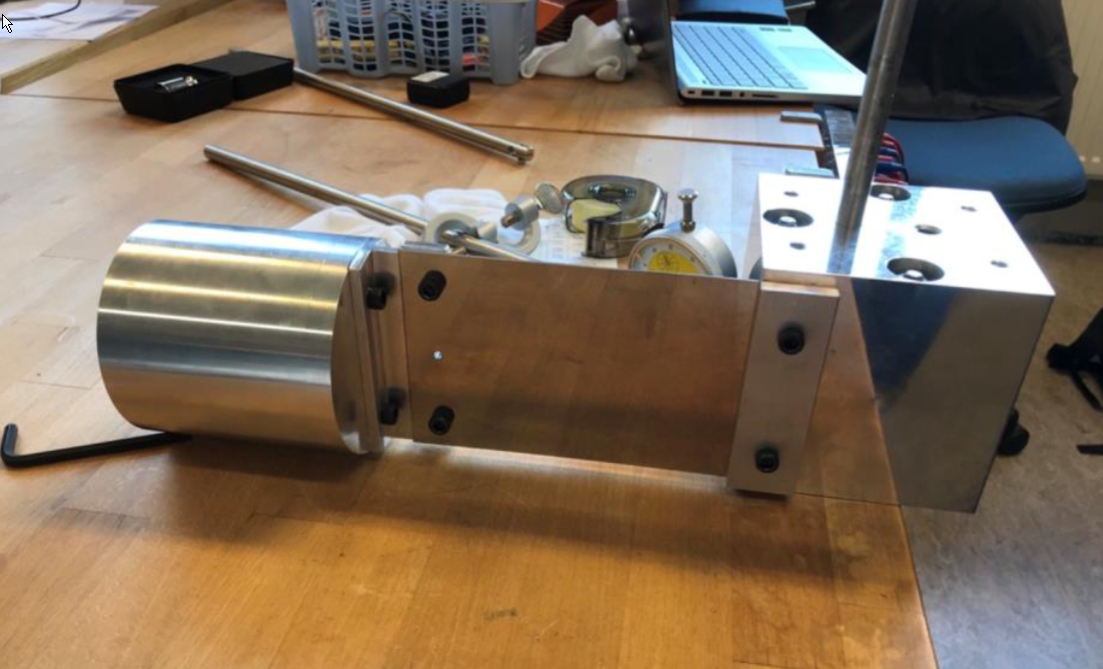
\includegraphics[width = .4\textwidth]{fig/oscillator_oppsett.png}
  \caption{Oppsett av harmonisk oscillator}
  \label{fig: oppsett oscillator}
\end{figure}

Vi spenner opp bladfjæren, men denne gangen vertikalt på aluminiums blokken, slik at den får svinge horisontalt (se \cref{fig: oppsett oscillator}). Vi finner massen til klossen ved å veie den på en balansevekt. Balansevekten har en usikkerhet på 0.1 g (se \cref{fig: datablad balansevekt}).
\paragraph{\bf Intensjon:} Måle hvor små masseendringer vi kan detektere ved å måle svingeperioden til klossen før og etter vi legger til en liten masse.  

\subsubsection{Måling}
Ved bruk av stoppeklokke tok vi tiden $t$ det tok for klossen å svinge 5 ganger. Usikkerheten i bruk av stoppeklokke anslo vi til å være på 0.2 sekunder. Vi gjennomførte dette 10 ganger og noterte tiden for hver gang (se \cref{tab: harmonic oscillator results}). 


\subsubsection{Beregninger}
Svingeperioden $\left<τ\right>$ fant vi ved bruk av formelen i \cref{eq: average period}. Vi brukte usikkerhetene i $\left<t\right>$ til å finne usikkerheten i $\left<τ\right>$. gitt ved \cref{eq: total time uncertainty}.
\begin{equation}\label{eq: average period}
    \left<τ\right> = \frac{\left<t\right>}{5}  
\end{equation}
\begin{equation}\label{eq: total time uncertainty}
    Δ\left<τ\right> = \frac{Δ\left<t\right>}{5}
\end{equation}
Videre bruker finner vi minste masseendring vi kan måle ved bruk av formelen i \cref{eq: mass uncertainty alternative}. Deretter tester vi om dette stemmer med en bunke med binders med masse tilnærmet lik som $Δm$ og ser om vi klarer å detektere endring i svingetiden og hvorvidt denne endringen er større enn usikkerheten vår. Vi bruker samme metode med 5 svingninger målt 10 ganger som notert i \cref{tab: harmonic oscillator results}
. Til slutt finner vi dynamisk område. 

\subsection{Bladfjær og Laser}
\subsubsection{Oppsett}
\begin{figure}[h!]
  \centering
  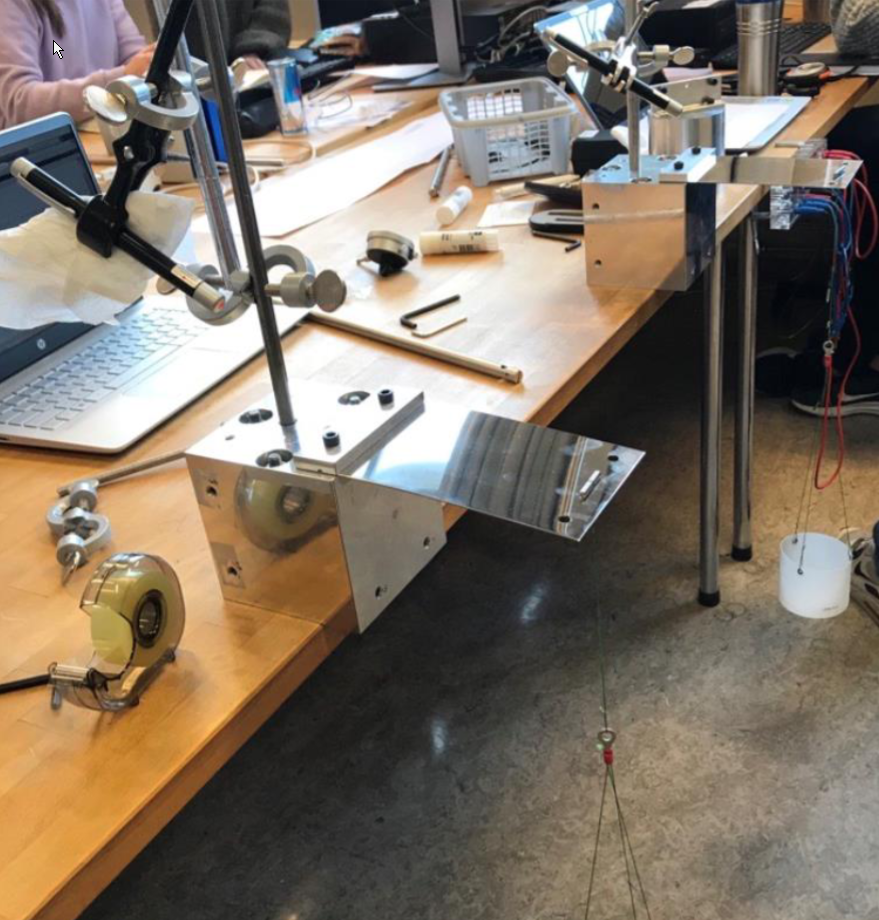
\includegraphics[width = .25\textwidth]{fig/laser_oppsett.png}
  \caption{Oppsett av bladfjær og laser}
  \label{fig: oppsett laser}
\end{figure}

I denne metoden er oppsettet for bladfjæren og kurven identisk som ved bruk av måleur i seksjon \ref{ssec: setup maaleur}. Forskjellen er at vi ikke bruker måleur, men har festet en laser på den vertikale stangen i aluminiums klossen som sett i \cref{fig: oppsett laser}. Vi legger på aluminiums blokken med litt ekstra vekt og peker laseren så langt ute på bladfjæren som mulig. Da sikrer vi oss at alle målinger kan gjennomføres og at vi får størst mulig spenn i posisjonen til laseren. Videre henger vi opp ark på veggen der laseren vil treffe slik at vi kan markere treffpunkt for laser og senere måle avstanden. 
\paragraph{\bf Intensjon:}
Laseren som peker på bladfjæren vil reflekteres av flaten og lyse på veggen noen meter unna. Når vi legger på mer vekt vil bladfjæreren trekkes nedover og laseren vil reflekteres lavere på veggen, jo mer vekt vi har på. Dette lar oss gjøre en lineærtilpassingen mellom avstand fra nullpunkt, til punktet laseren peker $δl$ nå vi har på $x$ antall kg

\subsubsection{Måling}
Før vi begynner målingene må vi igjen kalibrere vekten vår. Vi bruker samme metode som sist vi brukte bladfjæren i \ref{ssec: measurement maaleur}. Vi noterer vekt og $δl$ i \cref{tab: maaleur and laser results}.

\subsubsection{Beregninger}
Vi merker oss at prikken til laseren har en diameter på ca. 1 cm som legger til en avlesning usikkerhet $Δl_a$ på 5 mm i vår evne til å måle $δl$. Ettersom laseren peker ganske langt ute på bladfjæren vipper den også litt når vi legger på vekt. Dette gir en instrumentell usikkerhet $Δl_i$ på 5 mm. Vi legger derfor til disse usikkerhetene i vår beregning av $δl$. Videre finner vi følsomheten $Δm$ ved \cref{eq: mass uncertainty}.


\newpage
\section{Resultater} \label{sec: results}
\subsection{Tabeller}
\begin{table}[!ht]
    \begin{minipage}[t]{.4\linewidth}
    \centering
        \begin{tabular}[t]{l|c|r} 
        \toprule
        $m\ [g]$\hspace{0.125cm} &$l\ [mm]$\hspace{0.125cm} &$δl\ [cm]$ \\ 
        \midrule 
        0    &9,28 &0     \\ 
        1    &9,26 &0,2   \\ 
        10   &9,22 &0,5   \\ 
        100  &8,84 &4,4   \\ 
        500  &7,15 &23,2  \\ 
        600  &6,72 &27,8  \\ 
        700  &6,26 &32,4  \\ 
        1000 &4,99 &46,0  \\ 
        1100 &4,57 &50,3  \\ 
        1200 &4,12 &54,8  \\ 
        1500 &2,87 &67,7  \\ 
        1600 &2,45 &72,1  \\ 
        1700 &2,01 &76,1  \\ 
        2000 &0,79 &89,0  \\ 
        2100 &0,37 &92,9  \\ 
        2110 &0,30 &93,3  \\ 
        2120 &0,25 &93,7  \\ 
        2130 &0,20 &98,2  \\ 
        2131 &0,20 &94,3  \\ 
        \bottomrule
    \end{tabular}
    \caption{Masse og resultater fra målingene med måleur og laser.}\label{tab: maaleur and laser results}
    \end{minipage}\hspace{.125cm}
    \begin{minipage}[t]{.4\linewidth}
      \begin{tabular}[t]{l|r|r}
    \toprule
    Måling\hspace{0.05cm} &$l$ [mm] &$δl$ [cm] \\  
    \midrule
    1 &0,18 &95.7 \\  
    2 &0,15 &95.7 \\  
    3 &0,14 &95.7 \\  
    4 &0,14 & -\\  
    5 &0,13 & -\\  
    \bottomrule
  \end{tabular}
  \caption{Utslag ved veiing av aluminiums lodd med måleur og laser}
  \label{tab: aluminum weight results}
  \end{minipage}
\end{table}

\begin{table}[!ht]
  \begin{minipage}[t]{.45\linewidth} 
    \centering
        \begin{tabular}[t]{l|r} 
        \toprule
        $t_n$ &tid [s] \\
        \midrule
        $t_1$ &2,10 \\        
        $t_2$ &1,94 \\        
        $t_3$ &1,99 \\        
        $t_4$ &1,96 \\        
        $t_5$ &2,02 \\        
        $t_6$ &2,07 \\        
        $t_7$ &2,06 \\        
        $t_8$ &2,12 \\        
        $t_9$ &2,03   \\        
        $t_{10}$ &2,04 \\
        \bottomrule
        \end{tabular}
    \caption{Tid for 5 svinginger for harmonisk oscillator}
    \label{tab: harmonic oscillator results}
  \end{minipage}
  \begin{minipage}[t]{.45\linewidth} 
    \centering
        \begin{tabular}[t]{l|r} 
        \toprule
        $t_n$ &tid [s] \\
        \midrule
        $t_1$ &2,04 \\        
        $t_2$ &2,04 \\        
        $t_3$ &2,03 \\        
        $t_4$ &2,05 \\        
        $t_5$ &2,11 \\        
        $t_6$ &2,11 \\        
        $t_7$ &1,97 \\        
        $t_8$ &2,03 \\        
        $t_9$ &1,88   \\        
        $t_{10}$ &2,01 \\
        \bottomrule
        \end{tabular}
    \caption{Tid for 5 svinginger for harmonisk oscillator med ekstra vekt}
    \label{tab: harmonic oscillator extra weight results}
  \end{minipage}
\end{table}

\begin{table}[!ht]
  \begin{minipage}[t]{.45\linewidth}
    \begin{tabular}[t]{l | r}
    \toprule
    Koeffisient &Verdi \\  
    \midrule
    a &-235 \\  
    b &2178 \\  
    $σ_a$ &0.32 \\  
    $σ_b$ &1.7 \\
    $Δl$ &0.013 mm \\
    m &2143 g \\ 
    $Δm$ &3.6 g \\
    \bottomrule
    \end{tabular}
    \caption{Koeffisienter og dets usikkerheter for lineær regresjon ved veiing av aluminums lodd ved et måling med måleur}
    \label{tab: linear regression coefficients maaleur}
  \end{minipage}
  \begin{minipage}[t]{.45\linewidth}
    \begin{tabular}[t]{l | r}
    \toprule
    Koeffisient &Verdi \\  
    \midrule
    a &22.65 \\  
    b &-17.66 \\  
    $σ_a$ &0.1086 \\  
    $σ_b$ &6.929 \\  
    $Δl$ &0.707 mm \\
    m &2150 g \\ 
    $Δm$ &20 g \\
    \bottomrule
    \end{tabular}
    \caption{Koeffisienter og dets usikkerheter for lineær regresjon ved veiing av aluminums lodd ved et måling med laser}
    \label{tab: linear regression coefficients laser}
  \end{minipage}
\end{table}

\newpage
\subsection{Bladfjær og Måleur}
\begin{figure}[!ht]
  \centering
  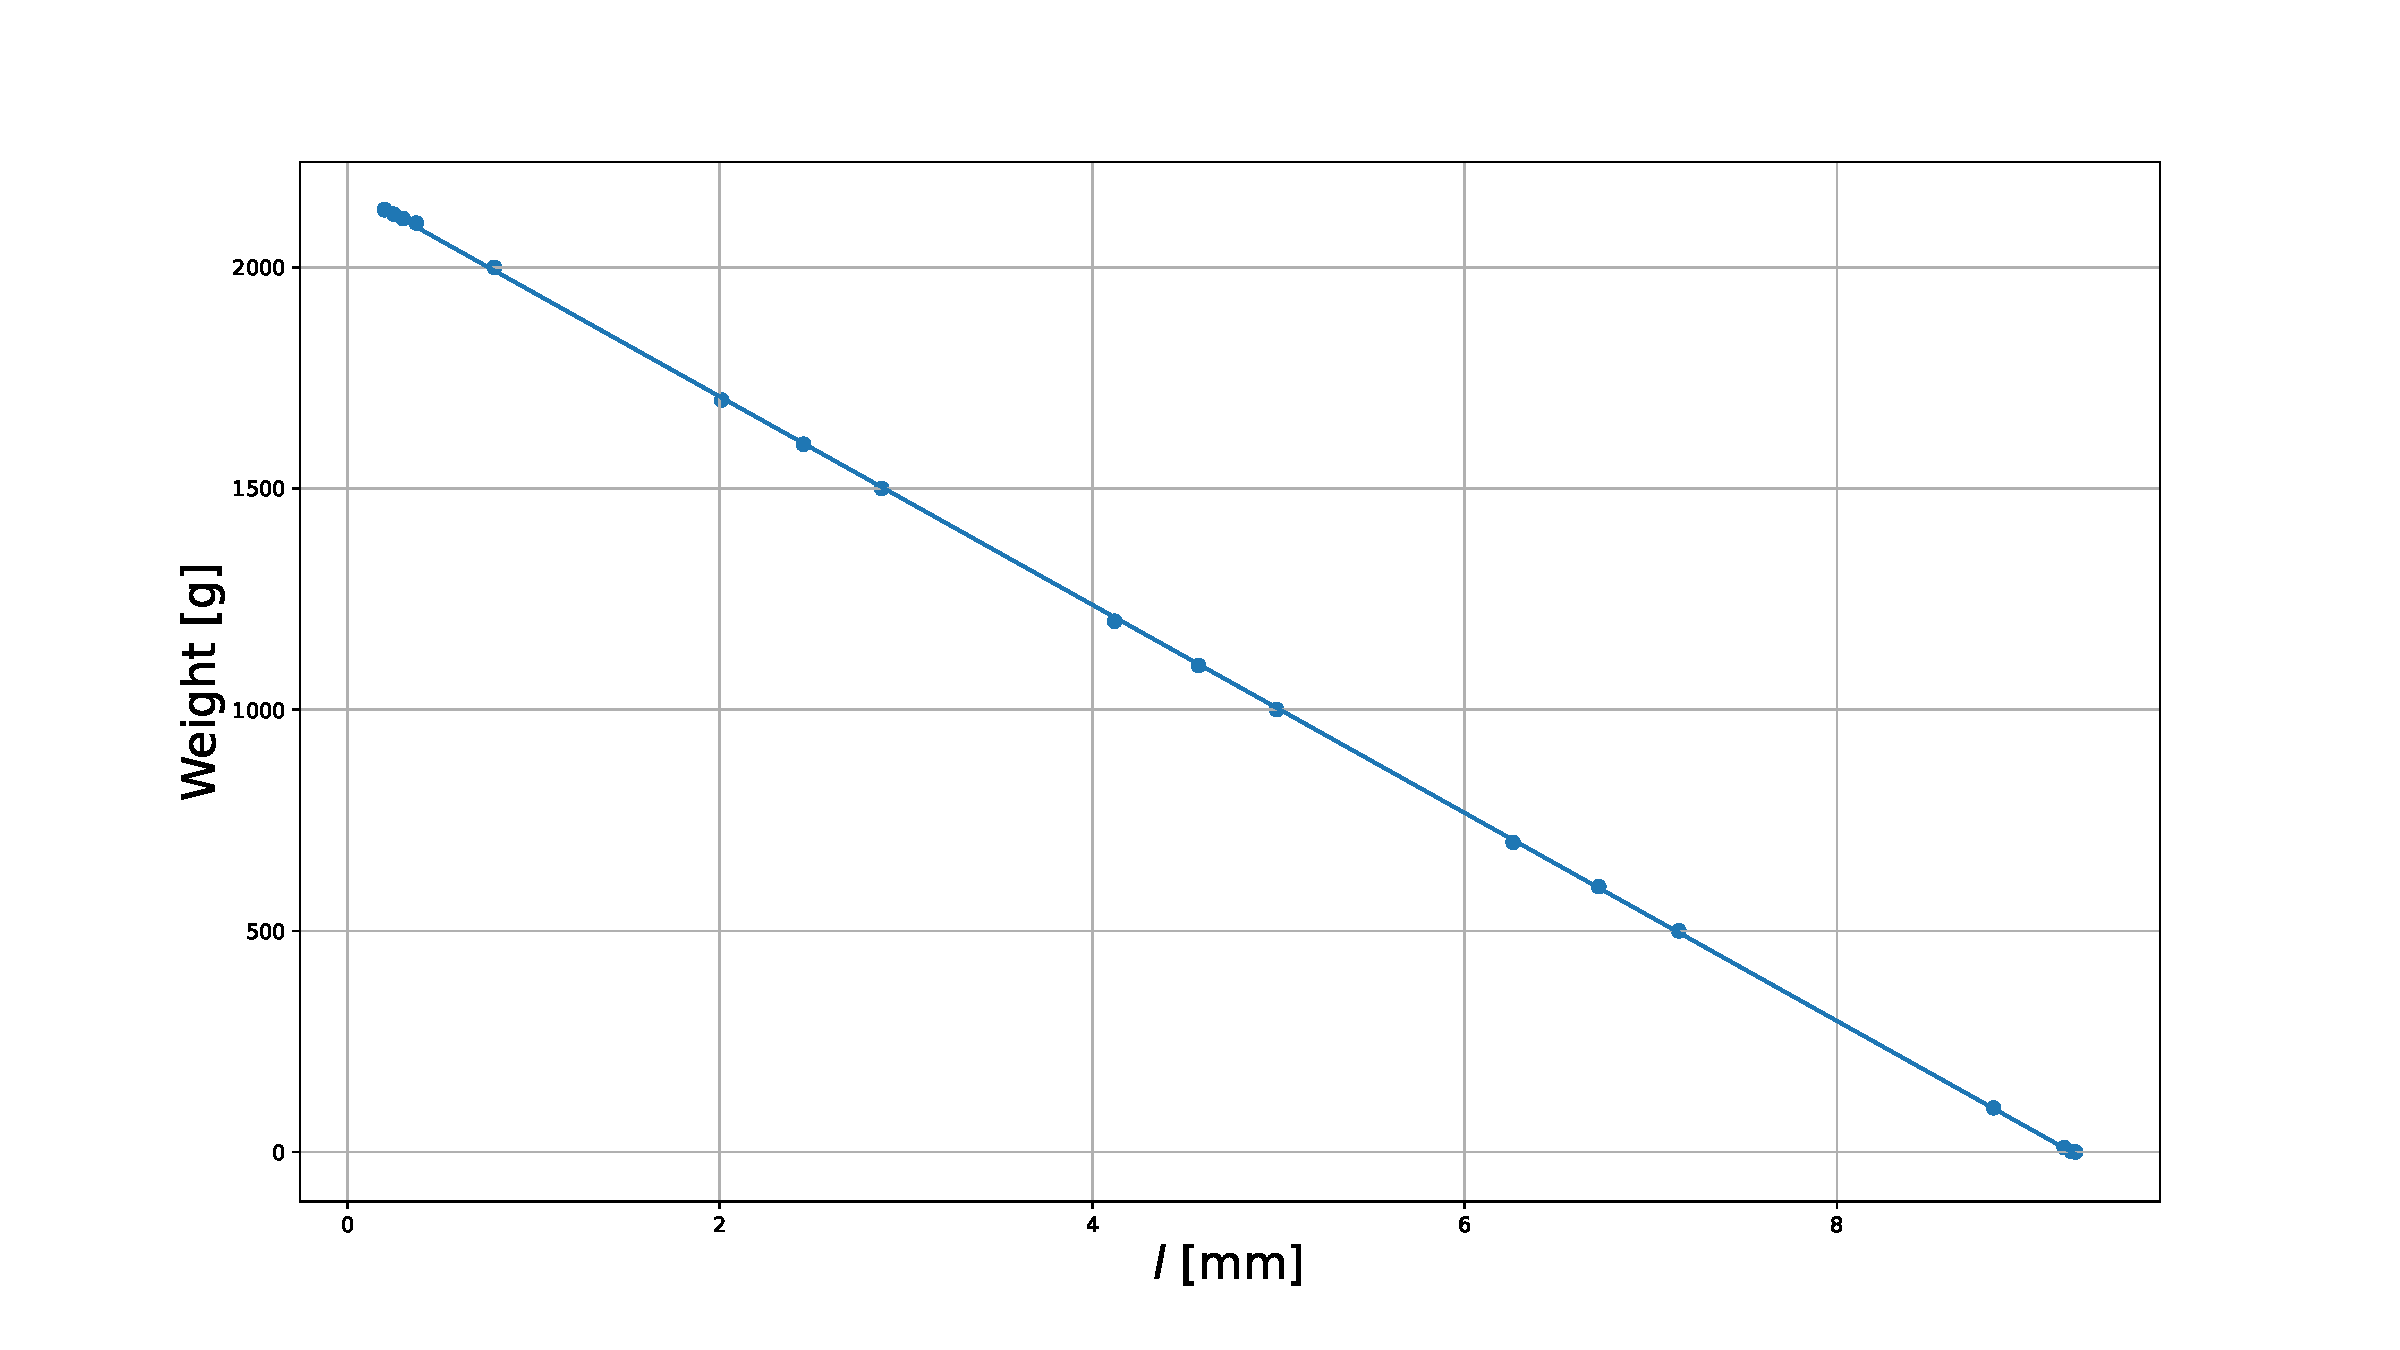
\includegraphics[width = .48\textwidth]{fig/linreg_maaleur.pdf}
  \caption{Lineær regresjon av måledata for bladfjær og måleur.}
  \label{fig: linreg maaleur}
\end{figure}


Se \cref{tab: linear regression coefficients maaleur} for numerisk beregnede verdier. 
Vi regner vi ut $Δl$ ved \cref{eq: total length uncertainty} og setter inn verdiene anslått og beregnet i \cref{ssec: calculations maaleur}
\begin{equation}\label{eq: total length uncertainty results}
  Δl = 0.013 \text{ mm}
\end{equation}

\subsection{Harmonisk Oscillator}
Etter å ha veid aluminiums loddet på balansevekten leser vi av en masse $m = 2143,4$ g. Vi regner også ut periodetiden $\left<τ_1\right>$ ved formelen \cref{eq: average period}. Vi finner standardavviket numerisk og får følgende resultat: 
\begin{equation}\label{eq: period result}
  \left<τ_1\right> = 0.407 ± 0.004 \text{ s}.
\end{equation}
Dette bruker vi videre til å finne $Δm$ via formel \cref{eq: mass uncertainty alternative} som gir følgende resultat:
\begin{equation}\label{eq: mass uncertainty alternative result}
  Δm = 39 \text{ g}.
\end{equation}
Vi samlet deretter en bunke med binders som vi veide på en digital vekt med en lesbarhet på 0,1 g (se \cref{fig: datablad balansevekt}) som ga oss en ny $\left<τ_2\right> = 0.405 ± 0.004$. 



\subsection{Bladfjær og Laser}
\begin{figure}[!ht]
  \centering
  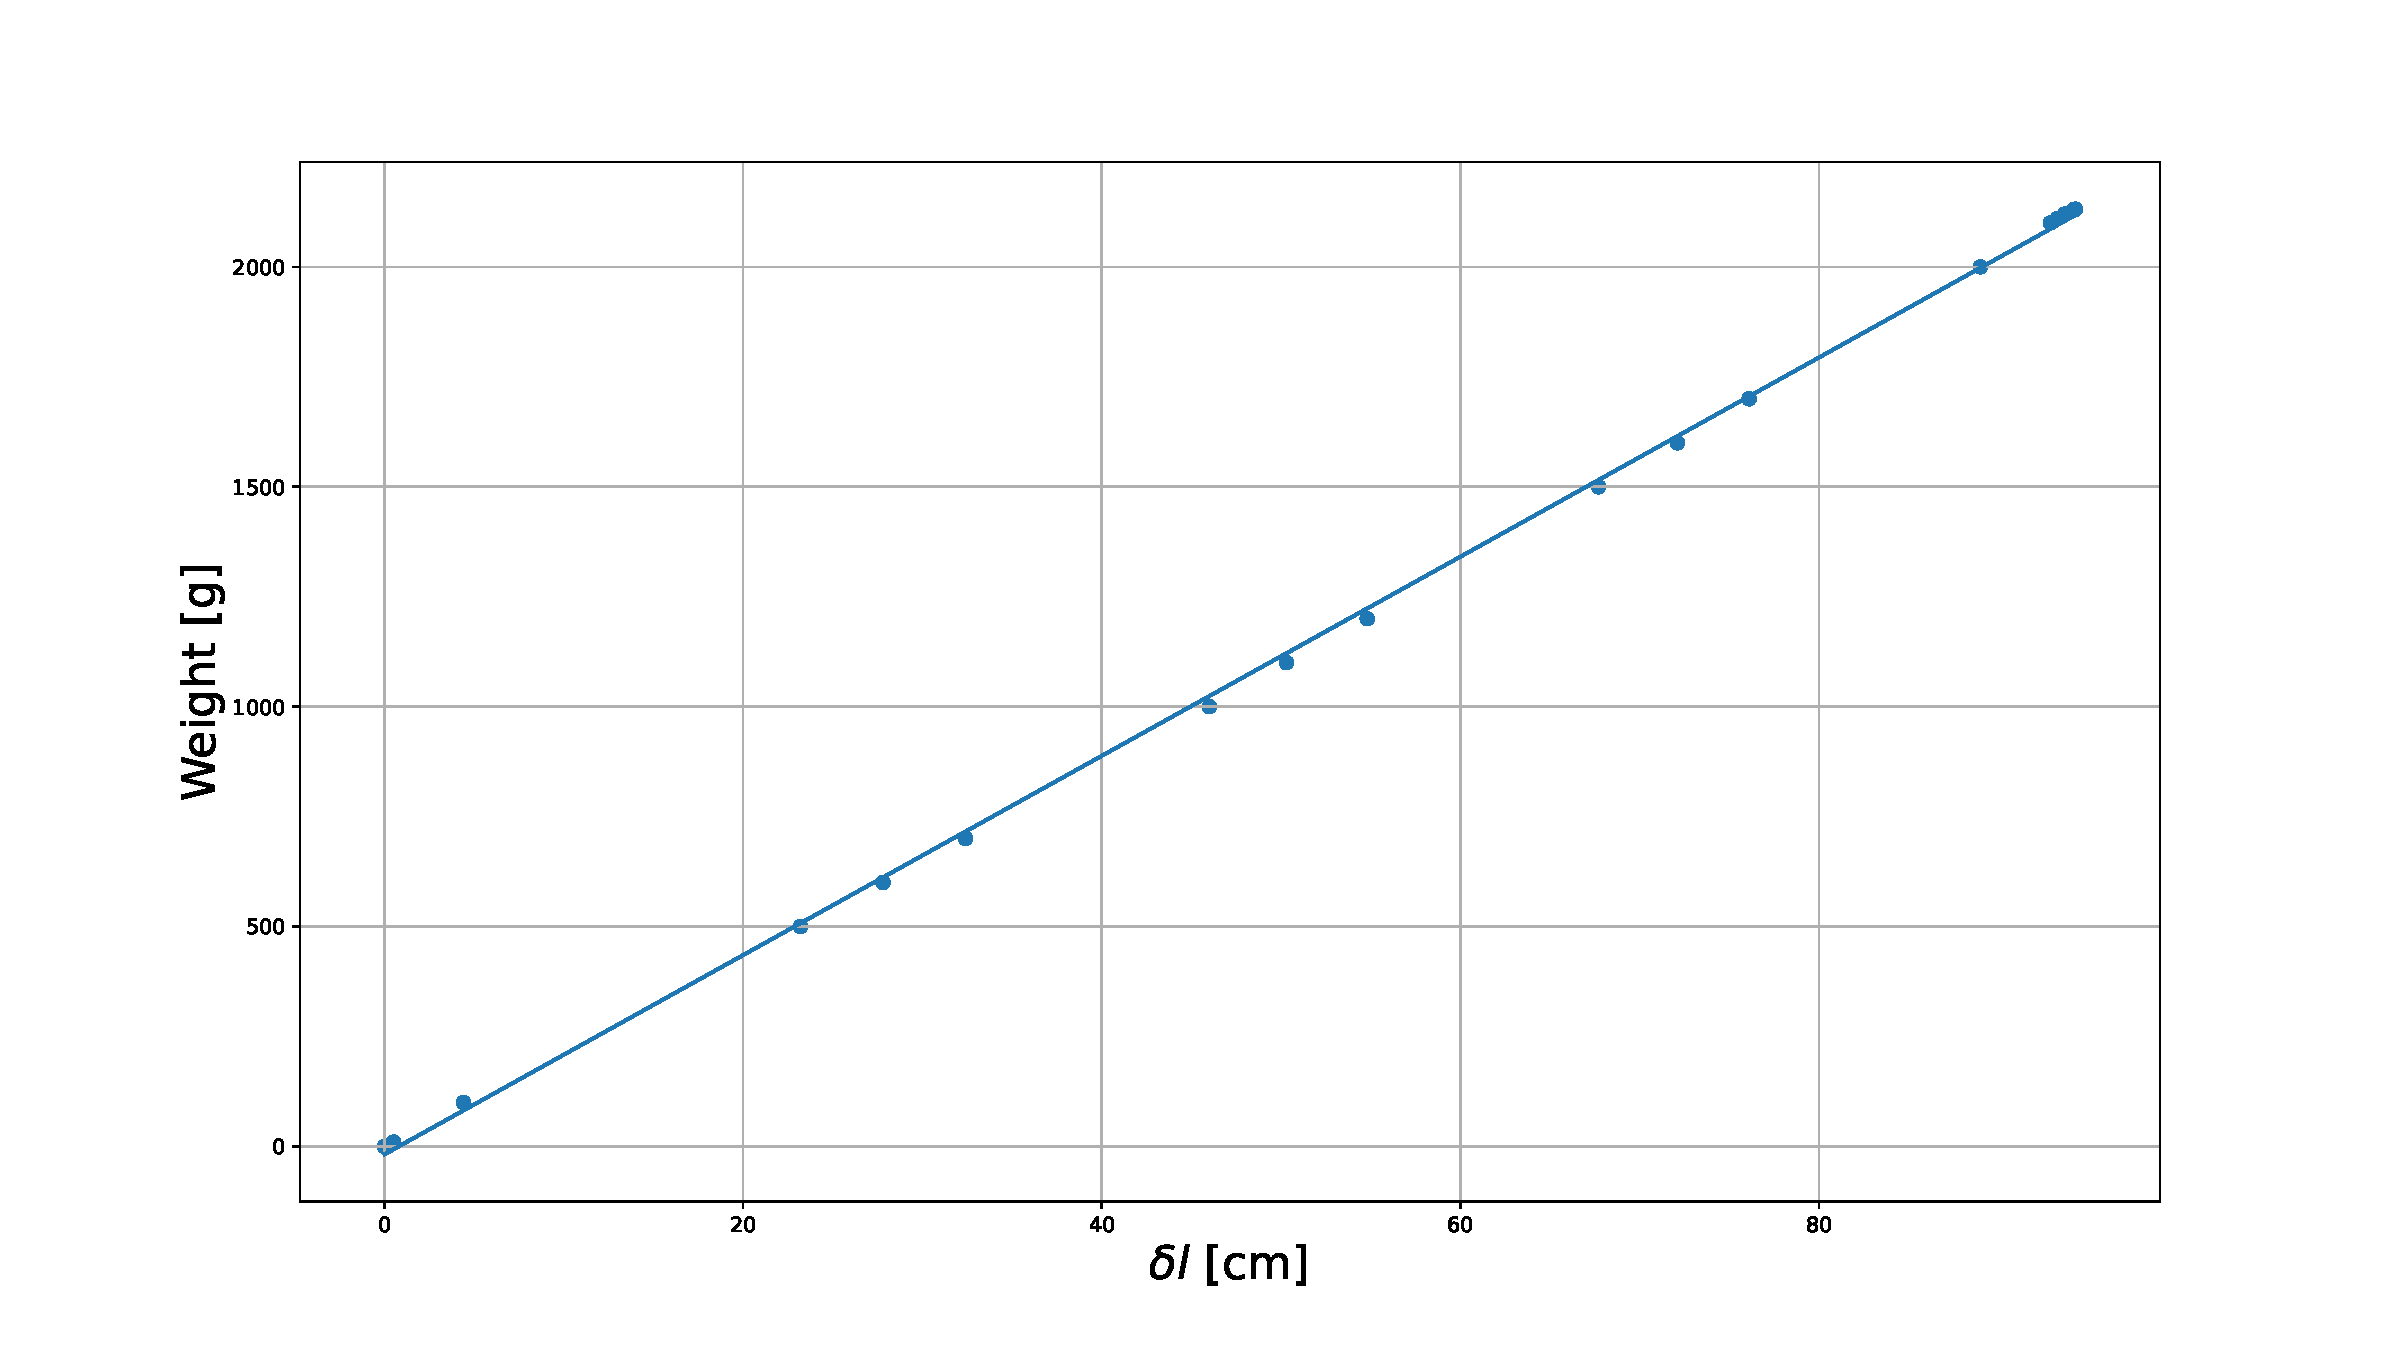
\includegraphics[width = 0.48\textwidth]{fig/linreg_laser.pdf}
  \caption{Lineær regresjon av måledata for bladfjær og laser.}
  \label{fig: linreg laser}
\end{figure}
Måledataen som sett i \cref{tab: aluminum weight results}, numeriske beregnede verdier i \cref{tab: linear regression coefficients laser} og formelen \cref{eq: total length uncertainty} gir oss følgende resultat for $Δl$:
\begin{equation}\label{eq: total length uncertainty results laser}
  Δl = \sqrt{0.5^2 + 0.5^2 + 0^2} = 0.707 \text{ mm}  
\end{equation}
Den numeriske lineærtilpassing hadde usikkerheter som sett i \cref{tab: linear regression coefficients laser}. Ved \cref{eq: mass uncertainty} beregner vi $Δm$.
\begin{equation}\label{eq: total mass uncertainty results laser}
  Δm = 26.00 \text{ g}
\end{equation}
Etter å ha veid aluminiums loddet på nytt etter å ha lagt til ekstra vekt på 10 g fikk vi et utslag 0.22 cm ekstra. 
Ved å bruke $δl$ målt ved veiing av aluminiums loddet, regnet vi numerisk en masse $m = 2140 ±26 $g. 


\section{Diskusjon} \label{sec: discussion}
\subsection{Bladfjær og Måleur}
Det første vi merket oss var den permanente deformasjonen i bladfjæren. Vi målte utslag ved 0 g og fant det til ha blitt redusert fra 9.28 til 9.22. Dette vil naturligvis gjøre lineærtilpassing mindre presis. Dette kan en tenke har påvirket aluminums loddet ettersom vi ser i \cref{tab: aluminum weight results} at utslaget minker for hver måling. Ettersom dette var det første forsøket for å måle masse, har det størst potensialet til å permanent deformere bladfjæren. Da er det naturlig det er her vi ser størst effekt. 

Likevel var det relativt nøyaktig resultater, i forhold til de andre metodene, som ble produsert. Hvis vi ønsker oss en presisjon på 1\% får vi et dynamisk område på tre størrelses fra 36 g til 2100. 


\subsection{Harmonisk Oscillator}
Det første vi legger merke til er at endringen i perioden er ca. det samme som usikkerheten i $\left<τ_2\right>$. Da er vår kalkulerte $Δm$ veldig nære følsomheten vi ser eksperimentelt. Her burde vi hatt flere målinger for å få en mer nøyaktig verdi. Likevel tyder dette på at vår teoretiske $Δm$ er i nærheten av den faktiske. Ettersom vi ikke har et friksjonsfritt system og permanent deformasjon av bladfjæren kan oppstå vil ikke periodetiden $τ$ være helt nøyaktig og vil endre seg over tid. Det er vanskelig å forutsi hvor mye dette påvirker lineærtilpassingen. Dette var grunnen til at vi valgte å bare ha 5 svingninger og flere målinger for å gjøre periodetiden mer konsekvent. 

En følsomhet på 39 g er relativt dårlig etter moderne standarder. Hvis vi ønsker oss en presisjon på 1\% får vi et dynamisk område på to størrelsesordener fra 360 g til 1800 g. 
For å forbedre eksperimentet kunne vi ha brukt et måleur med lenger nål samt lenger bladfjær av et materiale som letter går tilbake til gammel form. 

\subsection{Bladfjær og Laser}
En følsomhet på 26 g er ikke særlig mye bedre enn det vi fikk ved bruk av en harmonisk oscillator. Det er ca. 50 \% forbedring, men likevel relativt lite brukbart i en moderne verden, med tanke på at vårt dynamiske område. Eksperimentelt klarte vi å se forskjell på ned til 10 g, men dette var også innenfor standardavviket vårt. Vi ser i etterkant at det kunne lønt seg å ha laseren peke litt lenger unna enden på bladfjæren, ettersom laseren ville vært mer stabil. Dette observerte vi hos andre grupper. 
Enda en stor feilkilde er den permanente deformasjonen i bladfjæren som er ekstremt vanskelig å ta hensyn til. Ved høyere vekt vil bladfjæren deformeres mer og mer helt til utslaget ved 0 g blir større. 

Vi har antatt et lineært forhold mellom deformasjon og laserens posisjon på veggen. Dette må ikke nødvendigvis stemme ettersom dreiemomentet vekten har på bladfjæren vil reduseres jo mer vekt som legges på. Hvis vi ønsker oss en presisjon på 1\% får vi et dynamisk område på to størrelsesordener fra 260 g til 1900 g. For å forbedre eksperimentet kunne vi ha brukt en laser med enda skarpere fokus slik at den ikke vippet så mye opp og ned. Her kunne en også brukt en bladfjær av materiale som lettere går tilbake til gammel form. 



\section{Konklusjon} \label{sec: conclusion}
Det er en klar vinner av alle metodene vi har brukt i disse eksperimentene. Bladfjær med måleur ga definitivt best resultater med en hel størrelsesorden. Dette kan virke logisk ettersom måleuret er laget får høy presisjon ved små avstander. 


\newpage
\onecolumngrid
\section{Appendix} \label{sec: appendix}
\subsection{Datablader}
\begin{figure}[!ht]
  \centering
  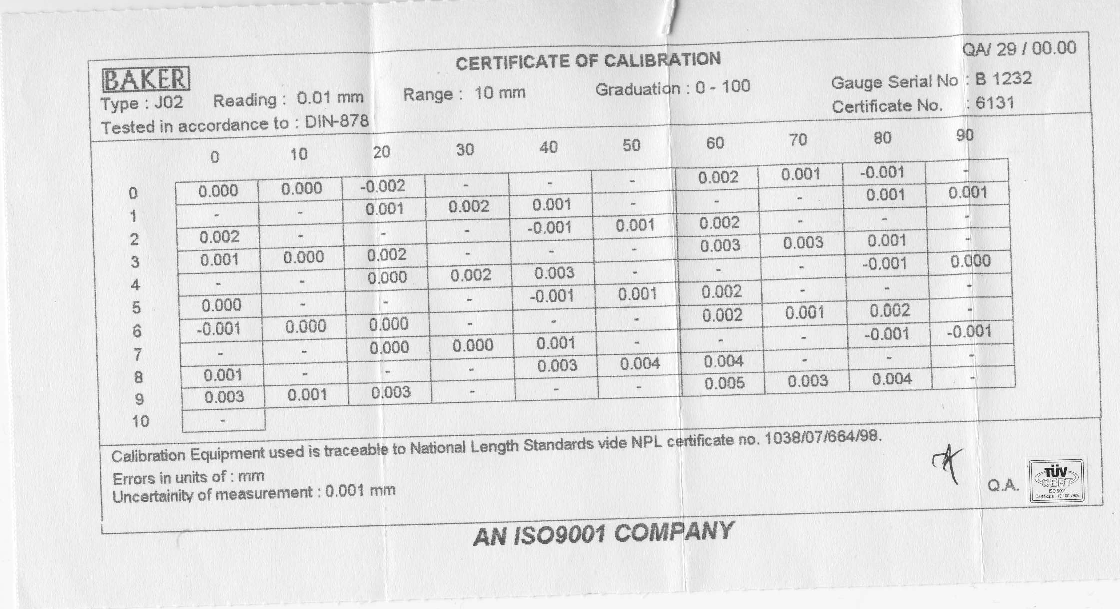
\includegraphics[width = \textwidth]{fig/Maaleur_B1232.PDF}
  \caption{Datablad for måleur B1232}
  \label{fig: datablad maaleur}
\end{figure}

\begin{figure}[!ht]
  \centering
  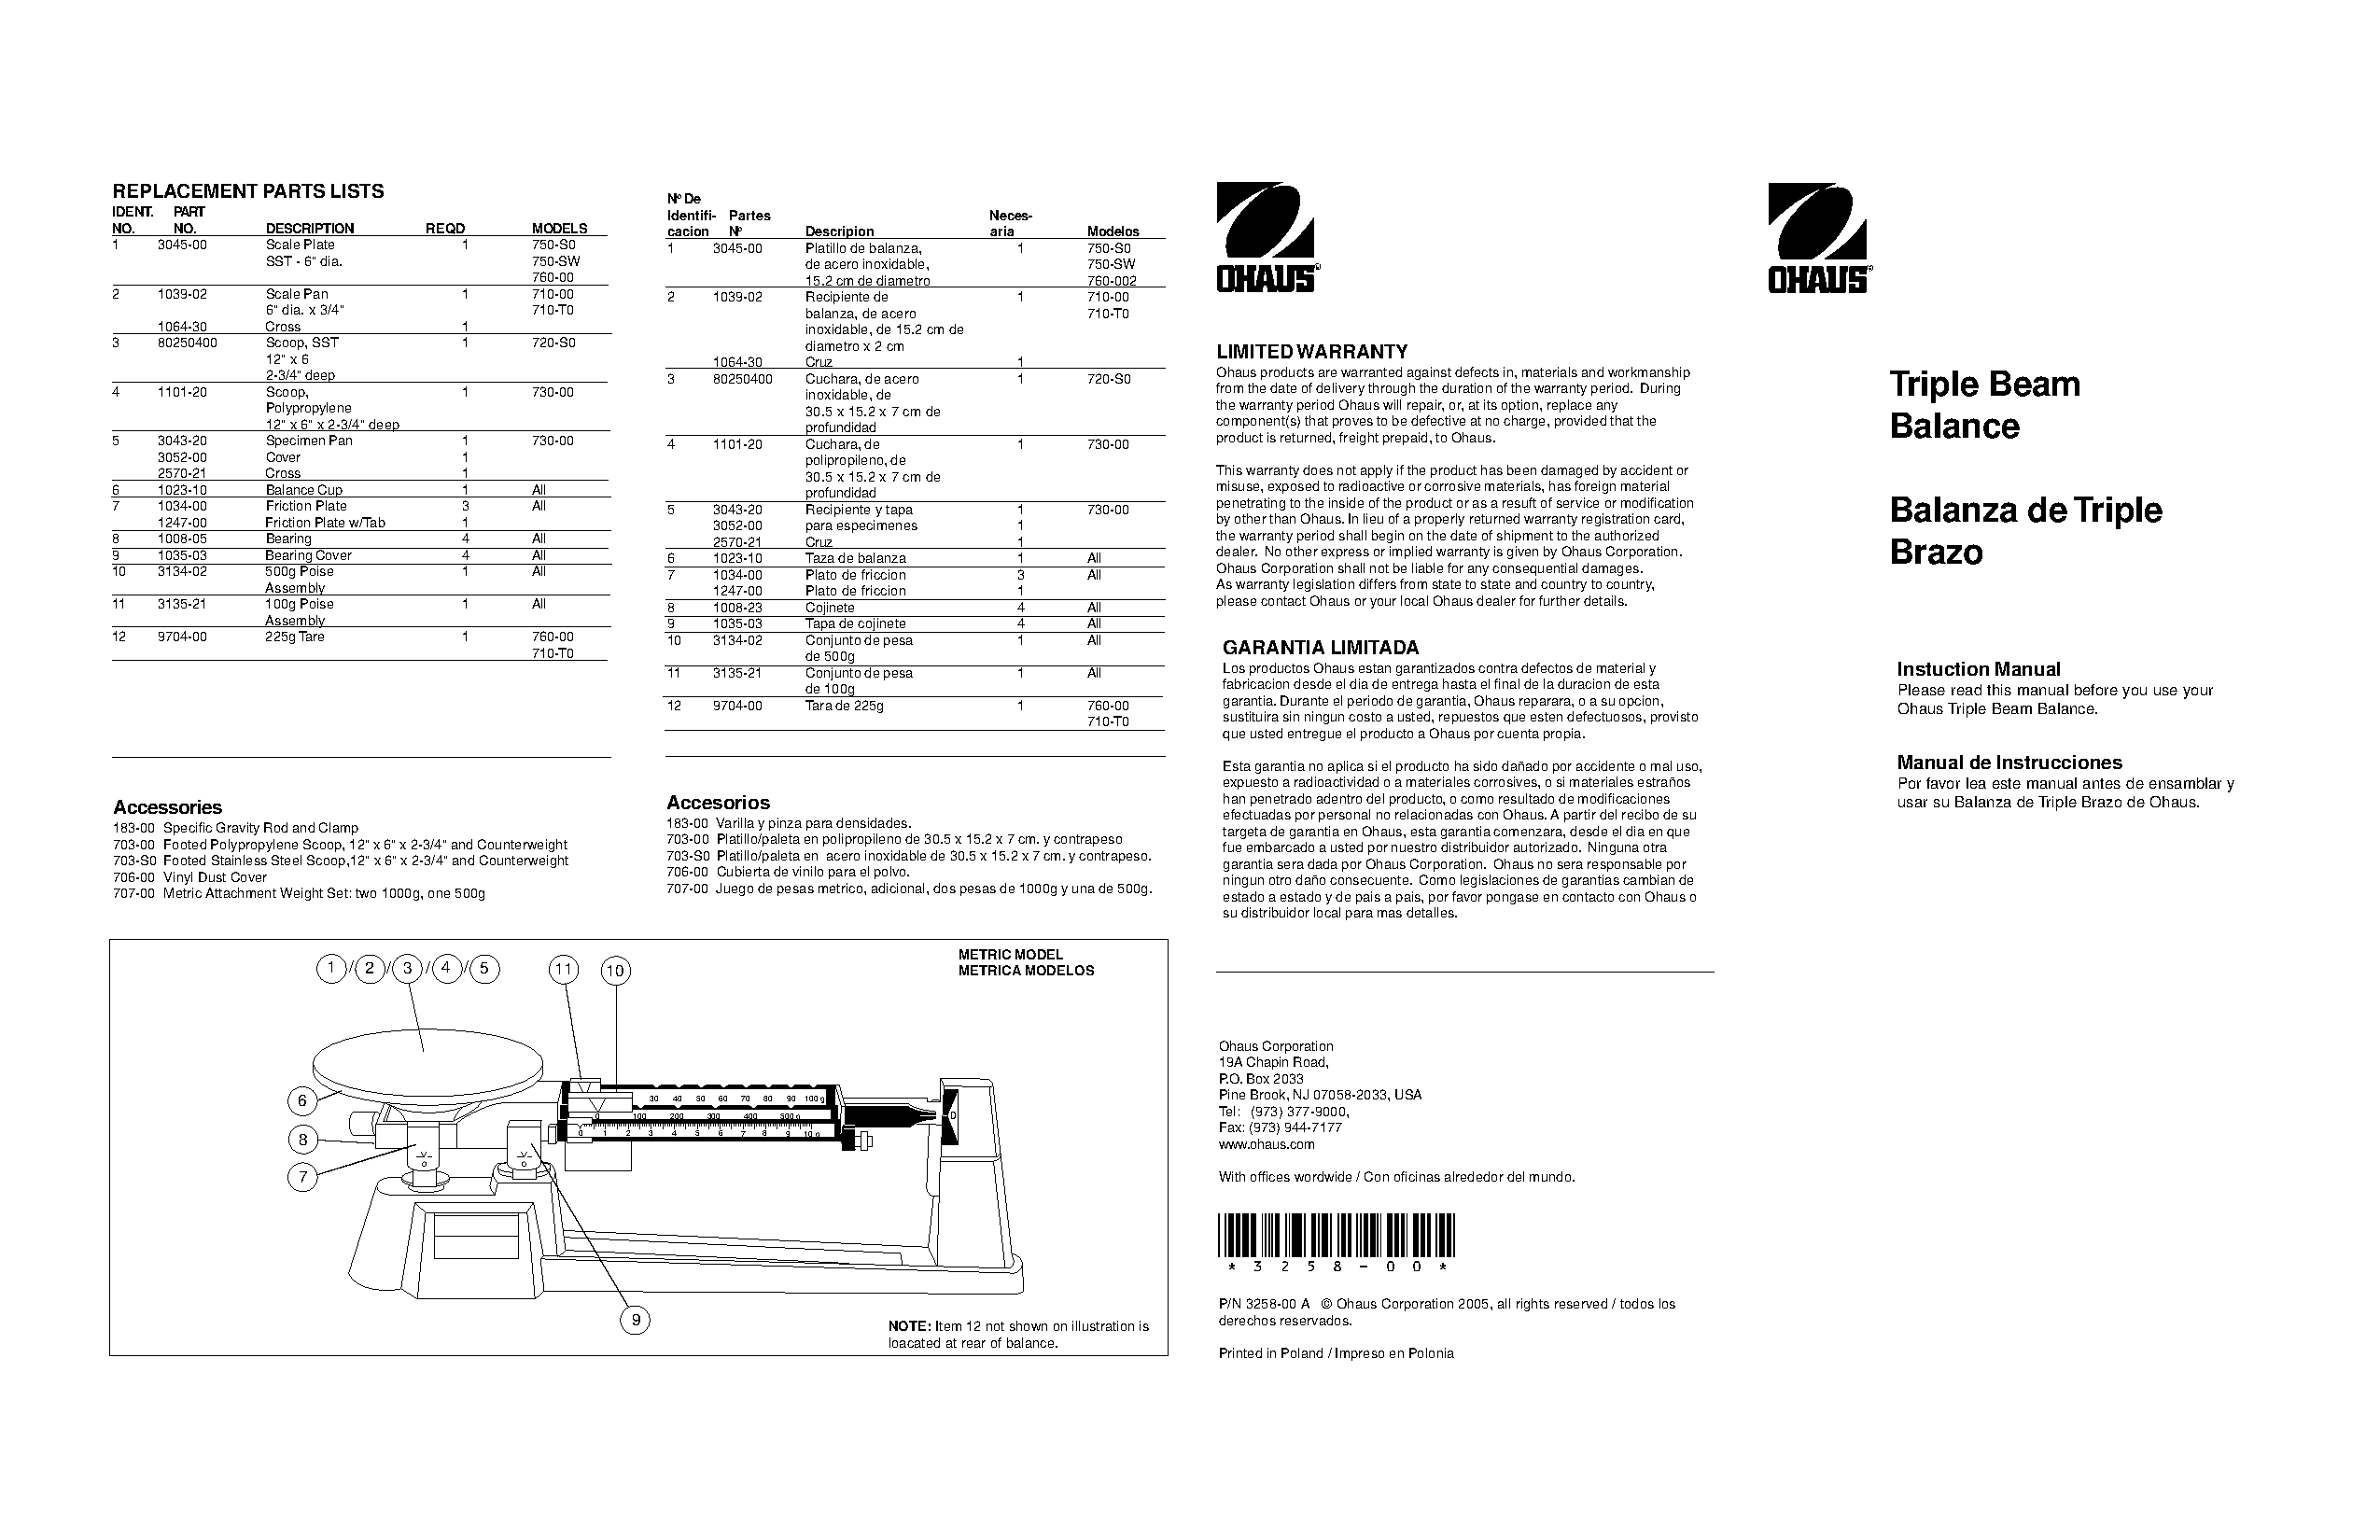
\includegraphics[width = .9\textwidth]{fig/balansevekt-ohaus-triple-beam-balance-manual.pdf}
  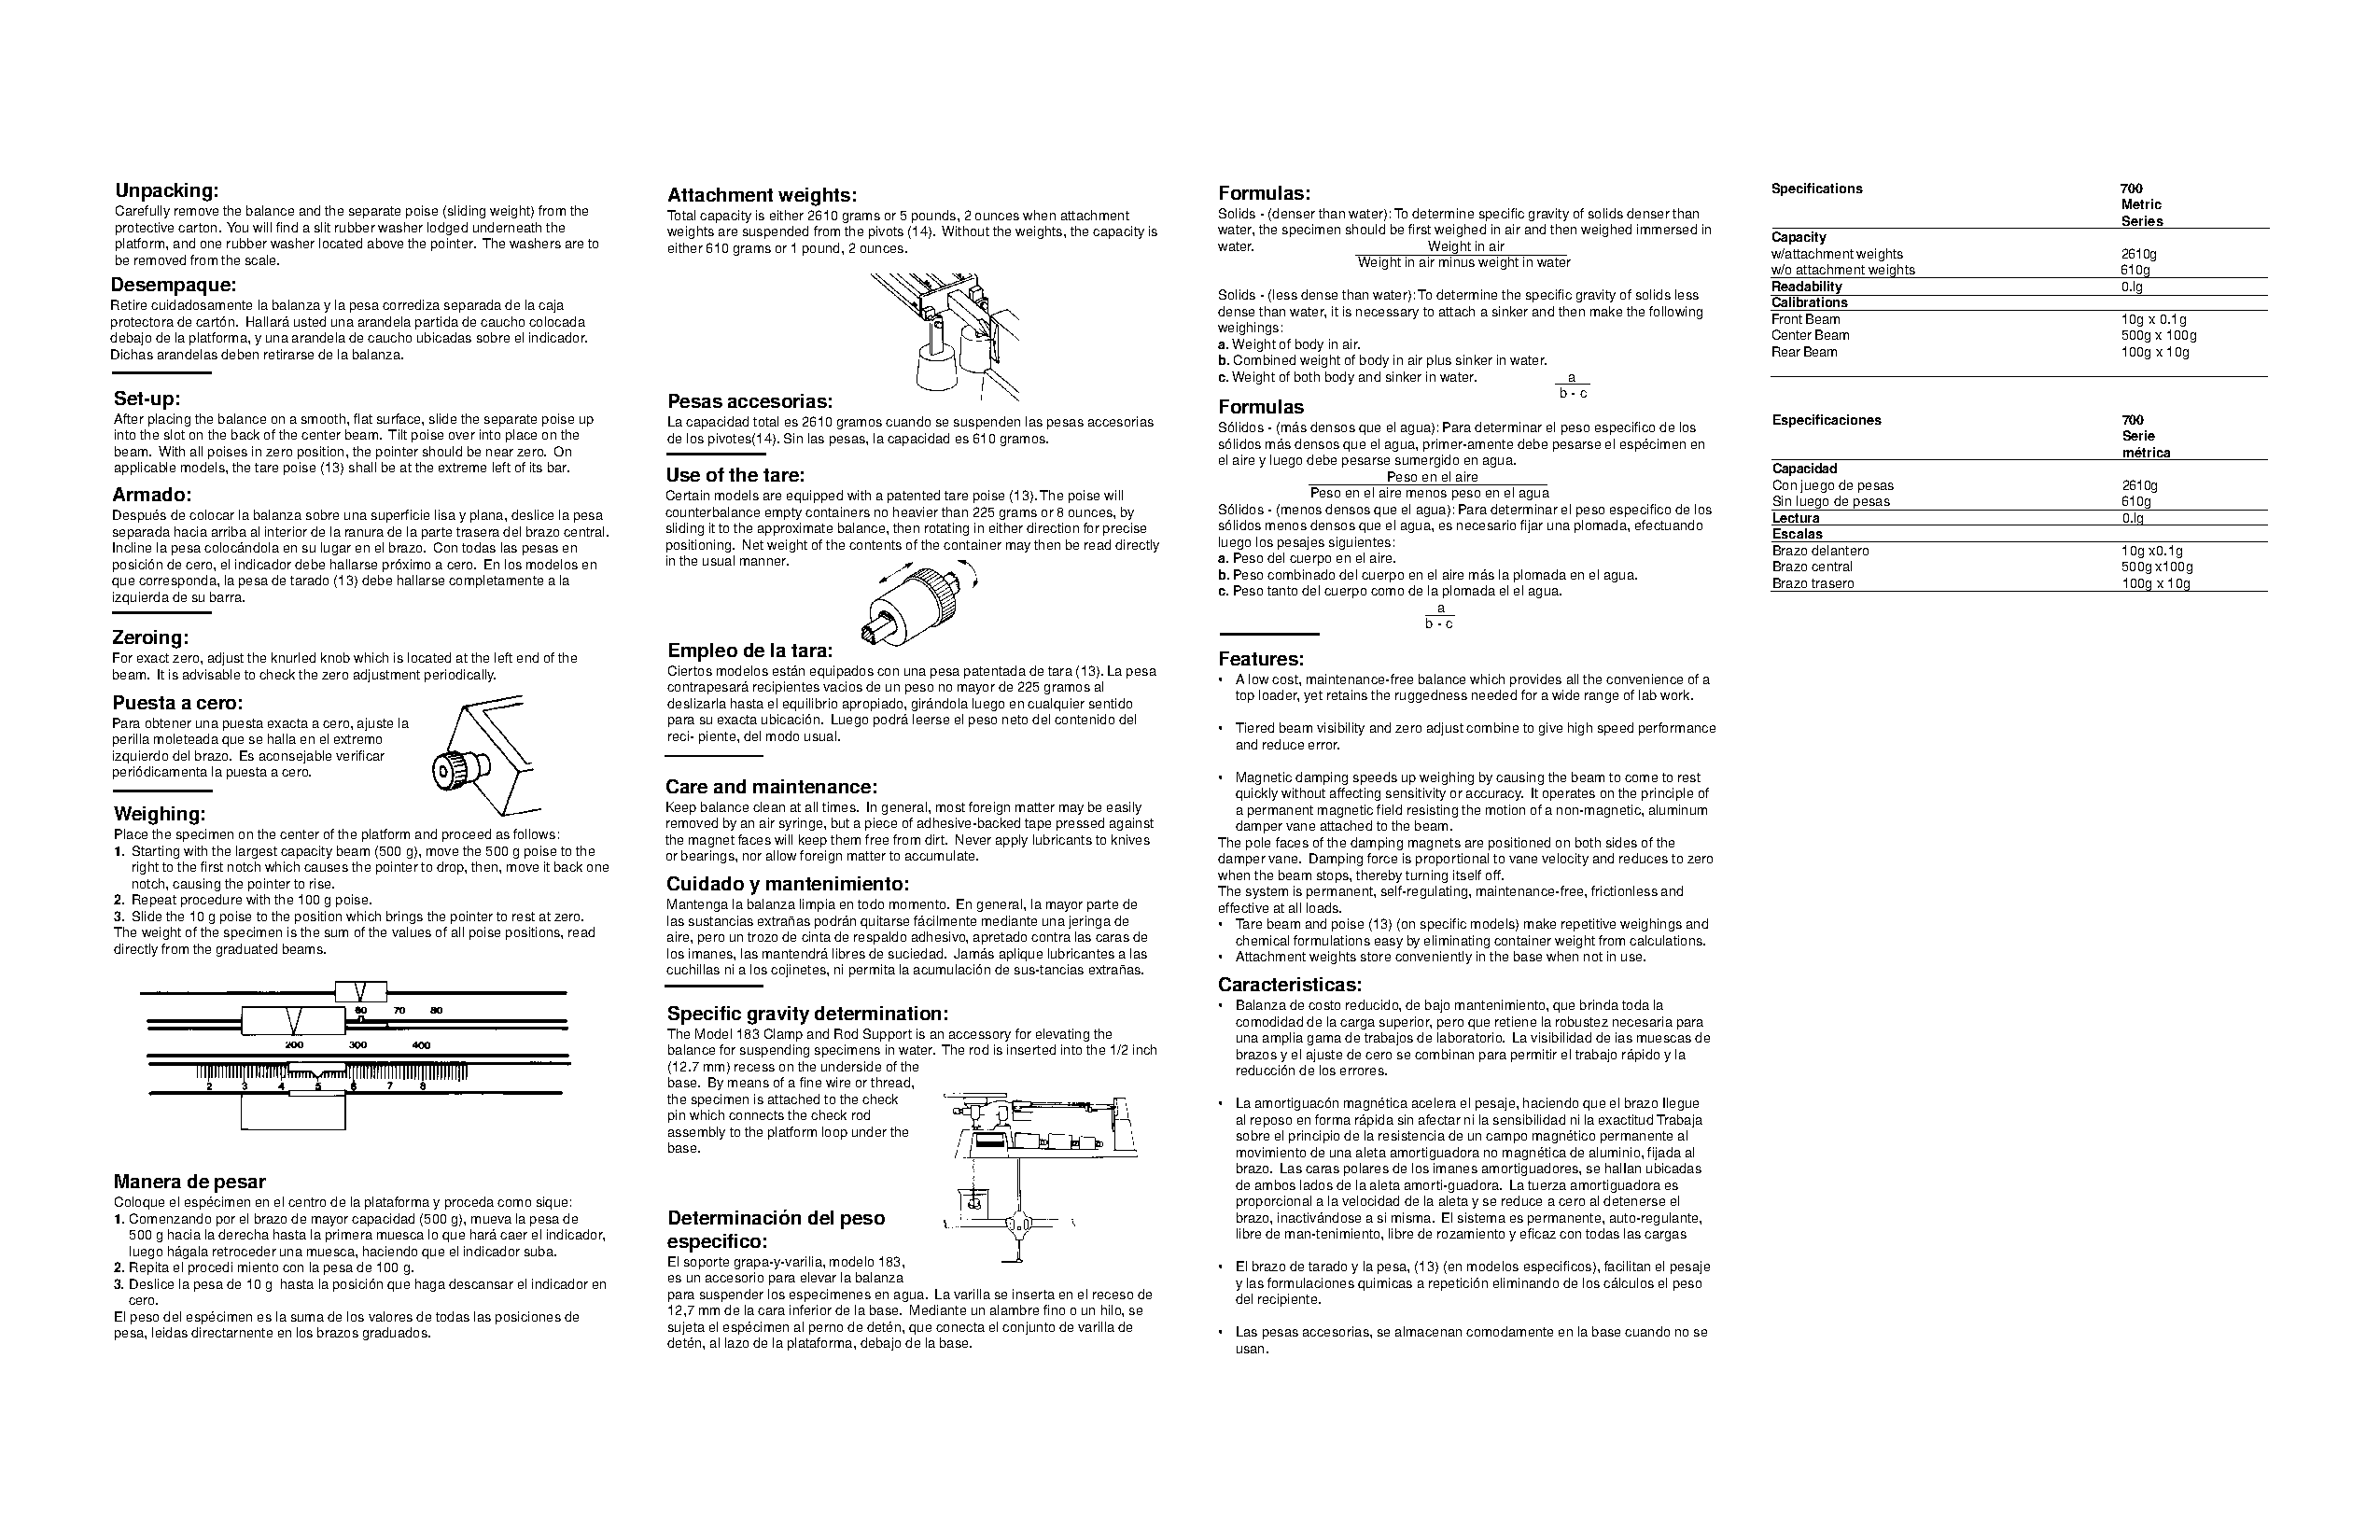
\includegraphics[width = .9\textwidth]{fig/balansevekt-ohaus-triple-beam-balance-manuals2.pdf}
  \caption{Datablad for balansevekt}
  \label{fig: datablad balansevekt}
\end{figure}

\begin{figure}[!ht]
  \centering
  
\includegraphics[width = .49\textwidth]{fig/proscalexc.pdf}
  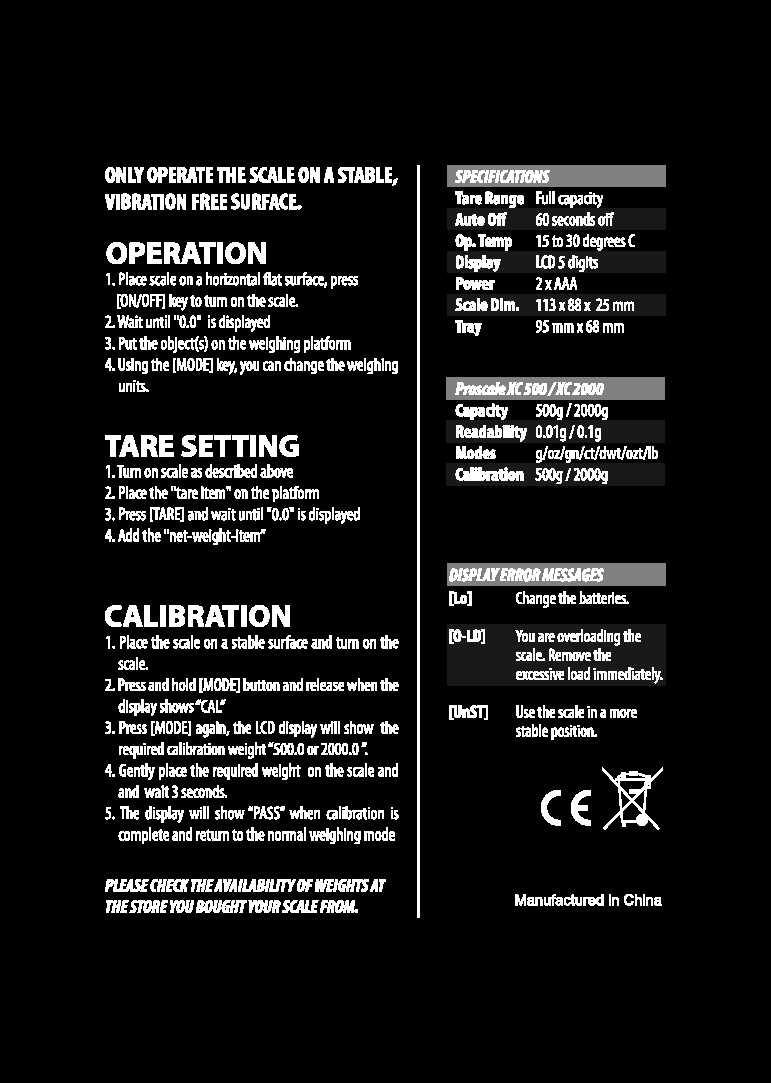
\includegraphics[width = .49\textwidth]{fig/proscalexc2.pdf}
  \caption{Datablad for digital vekt}
  \label{fig: datalad digital vekt}
\end{figure}

\newpage 
\subsection{Numeriske Beregninger}
\href{https://github.com/Oskar-Idland/FYS2150-Eksperimental-Fysikk/tree/Finished-Report-1/1%20Lab%20Raport}{Python filer på GitHub}

\end{document}